\subsubsection{Qu'est qu'une image}
Dans cette partie nous allons résoudre (1) à l'aide de discrétisation et de différences finies. Puis nous résoudrons celle-ci à l'aide des transformées de Fourier. \\
Avant de résoudre numériquement le problème, nous rappelons ce qu'est un image et le parcours d'une image.\\
Une image peut être représentée comme une succession de pixels. En traitement d'image, ce sont d'ailleurs sur ces pixels que le traitement est effectué. Leur modification entraîne la modification de l'image globale.Nous verrons donc une image comme la succession de pixels et nous pouvons la représenter comme une grille, dans laquelle chaque carré représente un pixel.  Schématiquement, nous pourrions donc découper notre image comme ci-dessous
    \begin{figure}[!htb]
        \centering
       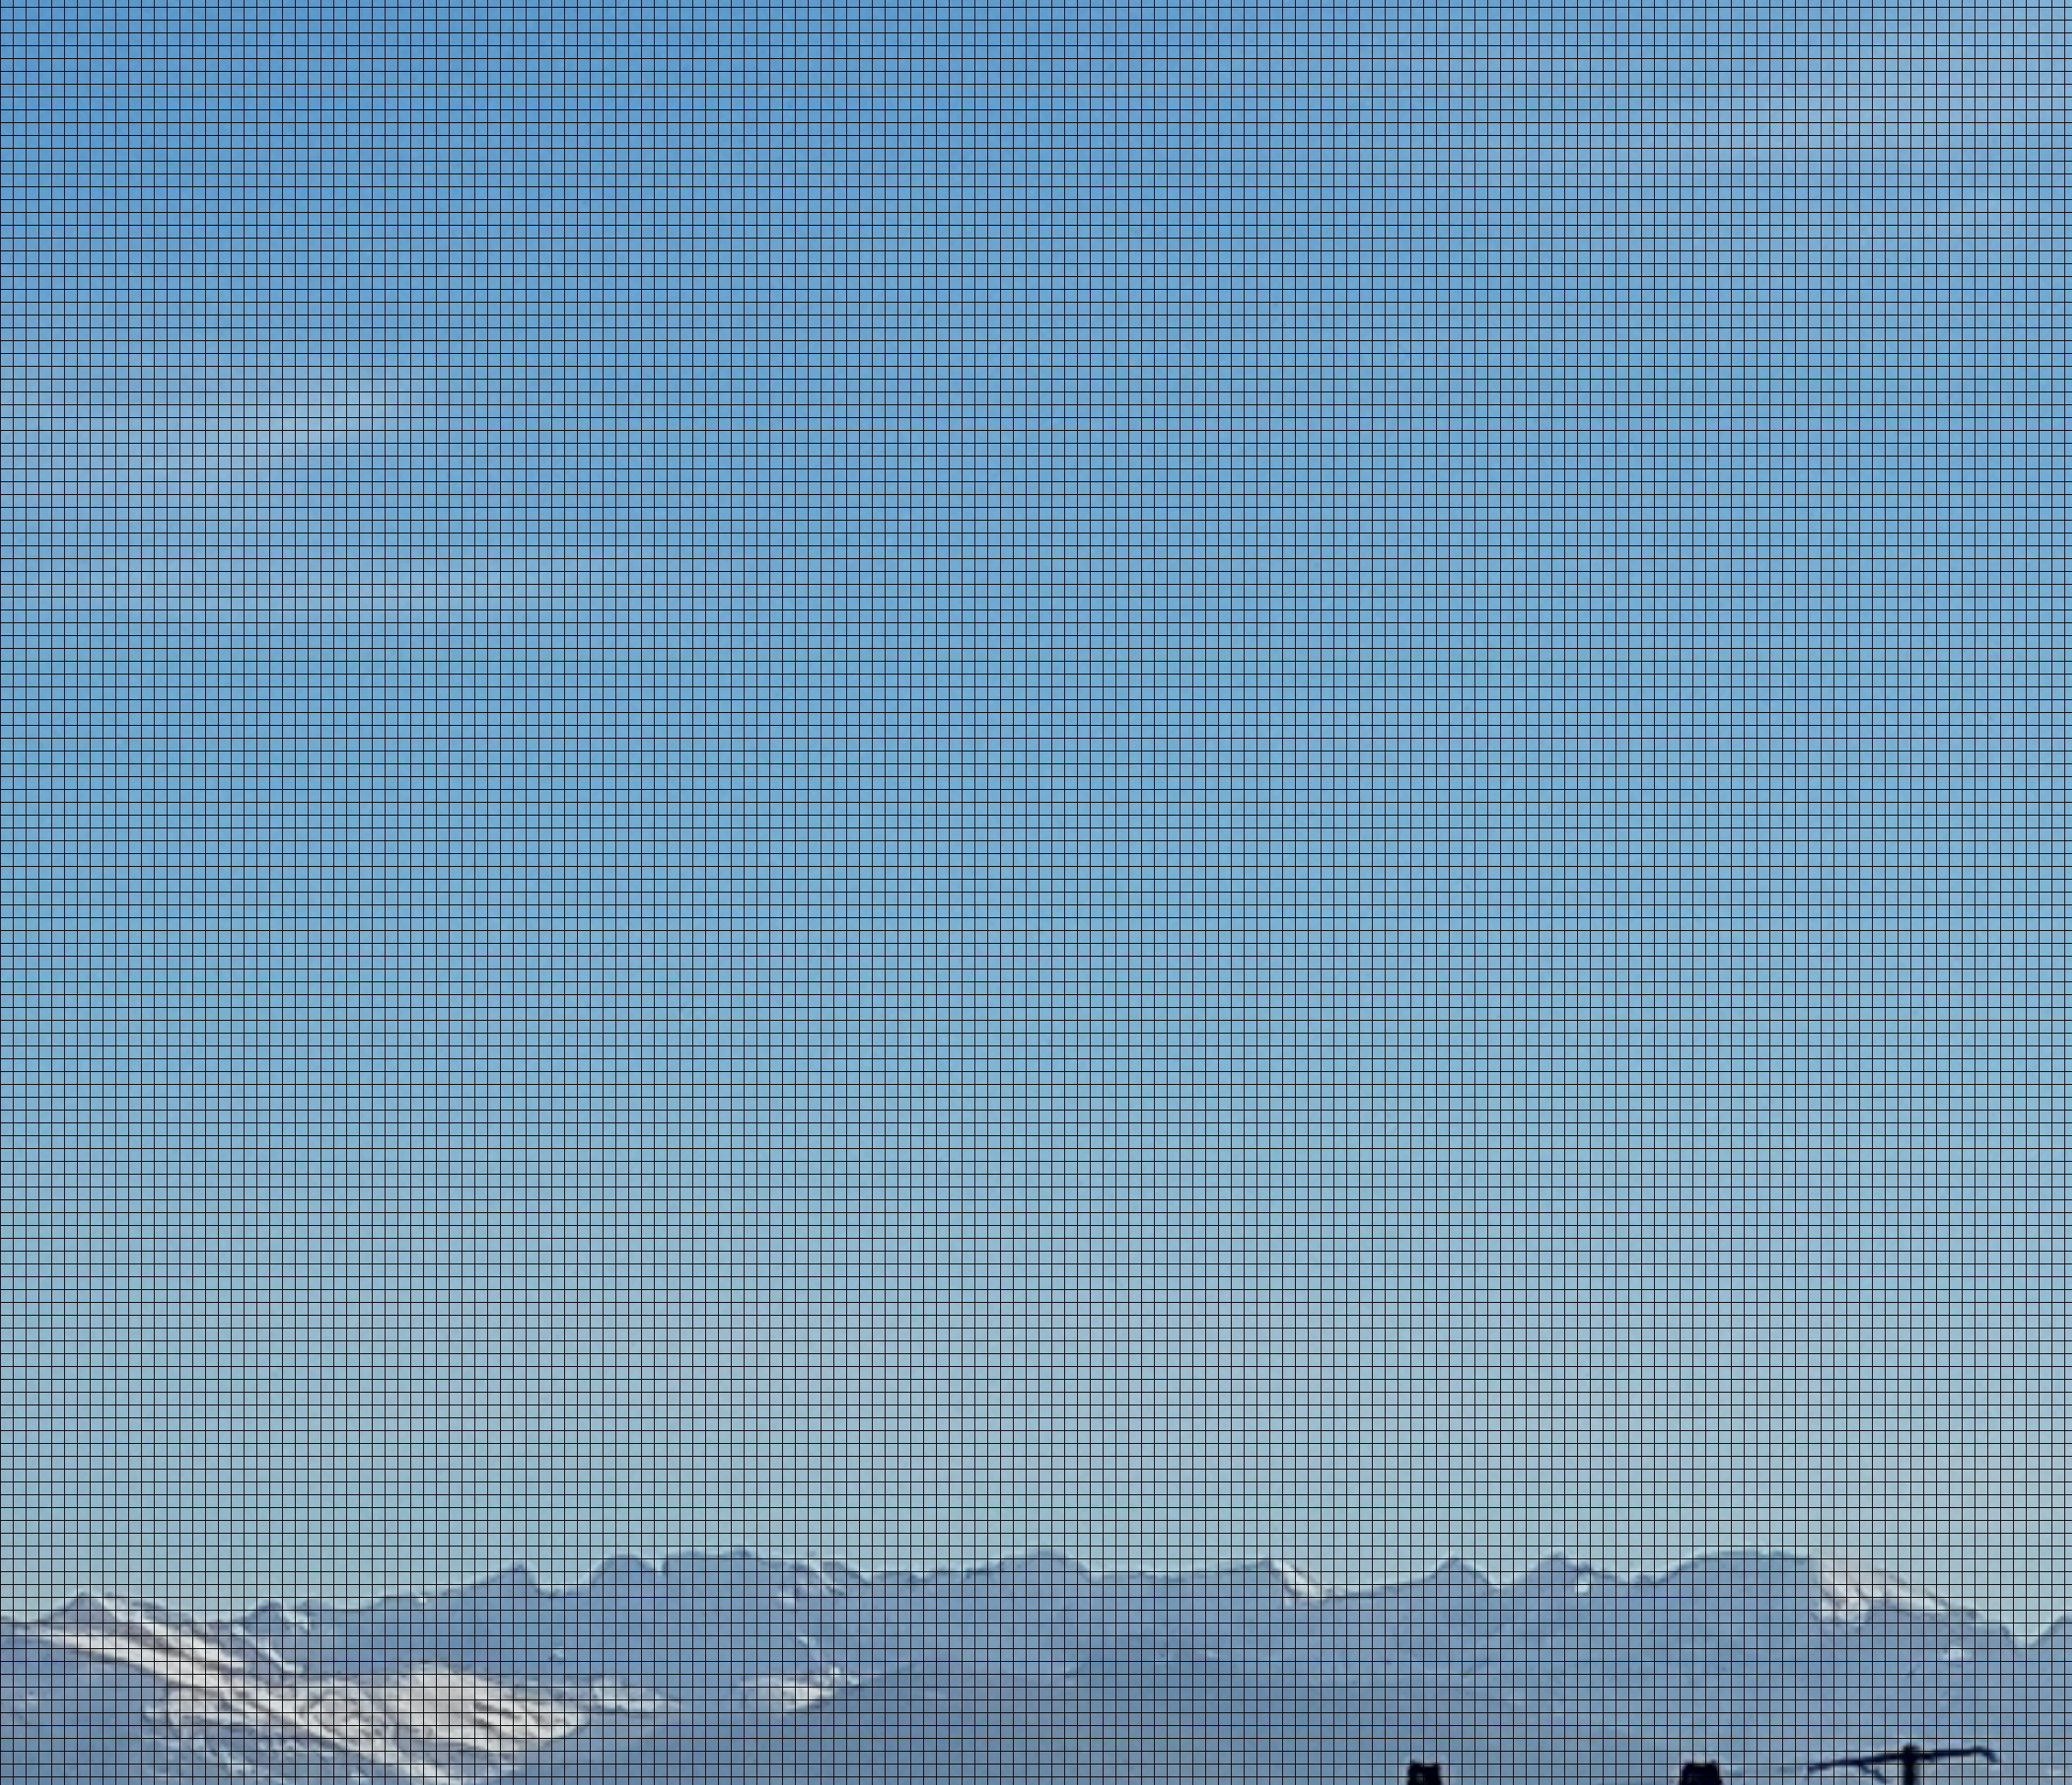
\includegraphics[scale = 0.07]{Images/Montagne_grille.jpg}
        \caption{Maillage d'une image}
        \label{fig:my_label}
    \end{figure}
Nous numéroterons les pixels suivant la règle suivante. Le premier pixel est situé en haut en gauche, puis il suffit de parcourir la grille comme ci-dessous : 

	\begin{figure}[!htb]
	\centering
	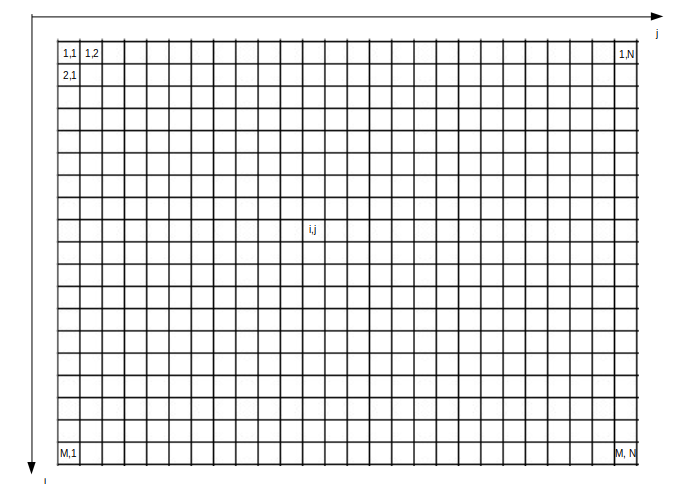
\includegraphics[scale=0.3]{Images/grille.png}
	\caption{Parcours d'une grille}
	\end{figure}
Les pas d'espaces sont donc égaux et valent 1. Dans la suite nous considérons que notre image est de taille $M \times N$.
\newpage

Rappelons que nous souhaitons résoudre l'équation de Poisson suivante : 
\begin{center}
\begin{equation*}
    \left \{
    \begin{aligned}
    \Delta I = \Delta S \ sur \ \Omega\\
    I = T \ sur \ \partial \Omega
    \end{aligned}
    \right.
\end{equation*}
\end{center}